% Options for packages loaded elsewhere
\PassOptionsToPackage{unicode}{hyperref}
\PassOptionsToPackage{hyphens}{url}
%
\documentclass[
]{book}
\usepackage{amsmath,amssymb}
\usepackage{lmodern}
\usepackage{iftex}
\ifPDFTeX
  \usepackage[T1]{fontenc}
  \usepackage[utf8]{inputenc}
  \usepackage{textcomp} % provide euro and other symbols
\else % if luatex or xetex
  \usepackage{unicode-math}
  \defaultfontfeatures{Scale=MatchLowercase}
  \defaultfontfeatures[\rmfamily]{Ligatures=TeX,Scale=1}
\fi
% Use upquote if available, for straight quotes in verbatim environments
\IfFileExists{upquote.sty}{\usepackage{upquote}}{}
\IfFileExists{microtype.sty}{% use microtype if available
  \usepackage[]{microtype}
  \UseMicrotypeSet[protrusion]{basicmath} % disable protrusion for tt fonts
}{}
\makeatletter
\@ifundefined{KOMAClassName}{% if non-KOMA class
  \IfFileExists{parskip.sty}{%
    \usepackage{parskip}
  }{% else
    \setlength{\parindent}{0pt}
    \setlength{\parskip}{6pt plus 2pt minus 1pt}}
}{% if KOMA class
  \KOMAoptions{parskip=half}}
\makeatother
\usepackage{xcolor}
\IfFileExists{xurl.sty}{\usepackage{xurl}}{} % add URL line breaks if available
\IfFileExists{bookmark.sty}{\usepackage{bookmark}}{\usepackage{hyperref}}
\hypersetup{
  pdftitle={Machine Learning for Quantitative Investment},
  pdfauthor={Fintelligence},
  hidelinks,
  pdfcreator={LaTeX via pandoc}}
\urlstyle{same} % disable monospaced font for URLs
\usepackage{color}
\usepackage{fancyvrb}
\newcommand{\VerbBar}{|}
\newcommand{\VERB}{\Verb[commandchars=\\\{\}]}
\DefineVerbatimEnvironment{Highlighting}{Verbatim}{commandchars=\\\{\}}
% Add ',fontsize=\small' for more characters per line
\usepackage{framed}
\definecolor{shadecolor}{RGB}{248,248,248}
\newenvironment{Shaded}{\begin{snugshade}}{\end{snugshade}}
\newcommand{\AlertTok}[1]{\textcolor[rgb]{0.94,0.16,0.16}{#1}}
\newcommand{\AnnotationTok}[1]{\textcolor[rgb]{0.56,0.35,0.01}{\textbf{\textit{#1}}}}
\newcommand{\AttributeTok}[1]{\textcolor[rgb]{0.77,0.63,0.00}{#1}}
\newcommand{\BaseNTok}[1]{\textcolor[rgb]{0.00,0.00,0.81}{#1}}
\newcommand{\BuiltInTok}[1]{#1}
\newcommand{\CharTok}[1]{\textcolor[rgb]{0.31,0.60,0.02}{#1}}
\newcommand{\CommentTok}[1]{\textcolor[rgb]{0.56,0.35,0.01}{\textit{#1}}}
\newcommand{\CommentVarTok}[1]{\textcolor[rgb]{0.56,0.35,0.01}{\textbf{\textit{#1}}}}
\newcommand{\ConstantTok}[1]{\textcolor[rgb]{0.00,0.00,0.00}{#1}}
\newcommand{\ControlFlowTok}[1]{\textcolor[rgb]{0.13,0.29,0.53}{\textbf{#1}}}
\newcommand{\DataTypeTok}[1]{\textcolor[rgb]{0.13,0.29,0.53}{#1}}
\newcommand{\DecValTok}[1]{\textcolor[rgb]{0.00,0.00,0.81}{#1}}
\newcommand{\DocumentationTok}[1]{\textcolor[rgb]{0.56,0.35,0.01}{\textbf{\textit{#1}}}}
\newcommand{\ErrorTok}[1]{\textcolor[rgb]{0.64,0.00,0.00}{\textbf{#1}}}
\newcommand{\ExtensionTok}[1]{#1}
\newcommand{\FloatTok}[1]{\textcolor[rgb]{0.00,0.00,0.81}{#1}}
\newcommand{\FunctionTok}[1]{\textcolor[rgb]{0.00,0.00,0.00}{#1}}
\newcommand{\ImportTok}[1]{#1}
\newcommand{\InformationTok}[1]{\textcolor[rgb]{0.56,0.35,0.01}{\textbf{\textit{#1}}}}
\newcommand{\KeywordTok}[1]{\textcolor[rgb]{0.13,0.29,0.53}{\textbf{#1}}}
\newcommand{\NormalTok}[1]{#1}
\newcommand{\OperatorTok}[1]{\textcolor[rgb]{0.81,0.36,0.00}{\textbf{#1}}}
\newcommand{\OtherTok}[1]{\textcolor[rgb]{0.56,0.35,0.01}{#1}}
\newcommand{\PreprocessorTok}[1]{\textcolor[rgb]{0.56,0.35,0.01}{\textit{#1}}}
\newcommand{\RegionMarkerTok}[1]{#1}
\newcommand{\SpecialCharTok}[1]{\textcolor[rgb]{0.00,0.00,0.00}{#1}}
\newcommand{\SpecialStringTok}[1]{\textcolor[rgb]{0.31,0.60,0.02}{#1}}
\newcommand{\StringTok}[1]{\textcolor[rgb]{0.31,0.60,0.02}{#1}}
\newcommand{\VariableTok}[1]{\textcolor[rgb]{0.00,0.00,0.00}{#1}}
\newcommand{\VerbatimStringTok}[1]{\textcolor[rgb]{0.31,0.60,0.02}{#1}}
\newcommand{\WarningTok}[1]{\textcolor[rgb]{0.56,0.35,0.01}{\textbf{\textit{#1}}}}
\usepackage{longtable,booktabs,array}
\usepackage{calc} % for calculating minipage widths
% Correct order of tables after \paragraph or \subparagraph
\usepackage{etoolbox}
\makeatletter
\patchcmd\longtable{\par}{\if@noskipsec\mbox{}\fi\par}{}{}
\makeatother
% Allow footnotes in longtable head/foot
\IfFileExists{footnotehyper.sty}{\usepackage{footnotehyper}}{\usepackage{footnote}}
\makesavenoteenv{longtable}
\usepackage{graphicx}
\makeatletter
\def\maxwidth{\ifdim\Gin@nat@width>\linewidth\linewidth\else\Gin@nat@width\fi}
\def\maxheight{\ifdim\Gin@nat@height>\textheight\textheight\else\Gin@nat@height\fi}
\makeatother
% Scale images if necessary, so that they will not overflow the page
% margins by default, and it is still possible to overwrite the defaults
% using explicit options in \includegraphics[width, height, ...]{}
\setkeys{Gin}{width=\maxwidth,height=\maxheight,keepaspectratio}
% Set default figure placement to htbp
\makeatletter
\def\fps@figure{htbp}
\makeatother
\setlength{\emergencystretch}{3em} % prevent overfull lines
\providecommand{\tightlist}{%
  \setlength{\itemsep}{0pt}\setlength{\parskip}{0pt}}
\setcounter{secnumdepth}{5}
\usepackage{booktabs}
\usepackage{amsthm}
\makeatletter
\def\thm@space@setup{%
  \thm@preskip=8pt plus 2pt minus 4pt
  \thm@postskip=\thm@preskip
}
\makeatother
\ifLuaTeX
  \usepackage{selnolig}  % disable illegal ligatures
\fi
\usepackage[]{natbib}
\bibliographystyle{apalike}

\title{Machine Learning for Quantitative Investment}
\author{Fintelligence}
\date{2022-01-29}

\begin{document}
\maketitle

{
\setcounter{tocdepth}{1}
\tableofcontents
}
\hypertarget{preface}{%
\chapter*{Preface}\label{preface}}
\addcontentsline{toc}{chapter}{Preface}

Welcome to the first edition of {Machine Learning for Quantitative Investment (ml4quant)}! This is an online book all about machine learning and data science methods in quantitative investment presented by \href{https://fintelligence-academy.github.io/}{Fintelligence Academy}: \url{https://fintelligence-academy.github.io/}.

The adoption of Machine Learning and Artificial Intelligence continues to progress from a niche activity to mainstream applications at an ever-accelerating pace in this Big Data era. Here at Fintelligence, we are embracing the ML in financial application.

In this book, we aim to walk through the \ldots.

Having quantitative research in mind, the intended audience is presumed interdisciplinary, fluent in mathematical notation, familiar with basic data science concepts. You may be surprised at the neglect of econometric/finance elements - we are confident to teach you the foundational knowledge of financial market along the reading journey. In addition, this book could be also interesting to those readers who are thinking of joining the quant workforce or data science community.

In another vein, this book also brings the mathematical foundations of basic machine learning concepts to the fore and collects the information in a single place so that a reader could learns both modern quantitative finance and machine learning. We assimilate and benefit core ideas from the two classical machine learning textbooks \emph{\href{https://www.statlearning.com/}{An Introduction to Statistical Learning} (ISL2)} and \emph{\href{https://hastie.su.domains/Papers/ESLII.pdf}{The Elements of Statistical Learning} (ESL)}, which are the best to-go reference books to learn machine learning. Here for ml4quant, we strive to strike a balance of difficulty in the middle level between the two books and season the topic with a new flavor of financial data science.

We genuinely hope that both the quantitative researchers and data scientists could enjoy reading this interdisciplinary book and find it helpful.

\begin{quote}
``The best time to plant a tree is twenty years ago. The second best time is now.'' - Chinese Proverb by \href{https://en.wikipedia.org/wiki/Wang_Bo_(poet)}{Poet Wang Bo}

``东隅已逝,桑榆非晚。''-王渤《滕王阁序》
\end{quote}

\hypertarget{intro}{%
\chapter{Introduction}\label{intro}}

Machine learning is the latest in a long line of attempts to distill human knowledge and reasoning into a form that is suitable for constructing computer automated systems. The enthusiastic practitioner who is interested to learn more about the magic behind successful machine learning algorithms currently faces a daunting set of pre-requisite knowledge:

\begin{itemize}
\item
  Programming languages and data analysis tools
\item
  Large-scale computation and the associated frameworks
\item
  Mathematics and statistics and how machine learning builds on it
\end{itemize}

Machine learning builds upon the language of mathematics to express concepts that seem intuitively obvious but that are surprisingly difficult to formalize. Once formalized properly, we can gain insights into the task we want to solve.

You can label chapter and section titles using \texttt{\{\#label\}} after them, e.g., we can reference Chapter \ref{intro}. If you do not manually label them, there will be automatic labels anyway, e.g., Chapter \ref{methods}.

Figures and tables with captions will be placed in \texttt{figure} and \texttt{table} environments, respectively.

\begin{Shaded}
\begin{Highlighting}[]
\FunctionTok{par}\NormalTok{(}\AttributeTok{mar =} \FunctionTok{c}\NormalTok{(}\DecValTok{4}\NormalTok{, }\DecValTok{4}\NormalTok{, .}\DecValTok{1}\NormalTok{, .}\DecValTok{1}\NormalTok{))}
\FunctionTok{plot}\NormalTok{(pressure, }\AttributeTok{type =} \StringTok{\textquotesingle{}b\textquotesingle{}}\NormalTok{, }\AttributeTok{pch =} \DecValTok{19}\NormalTok{)}
\end{Highlighting}
\end{Shaded}

\begin{figure}

{\centering 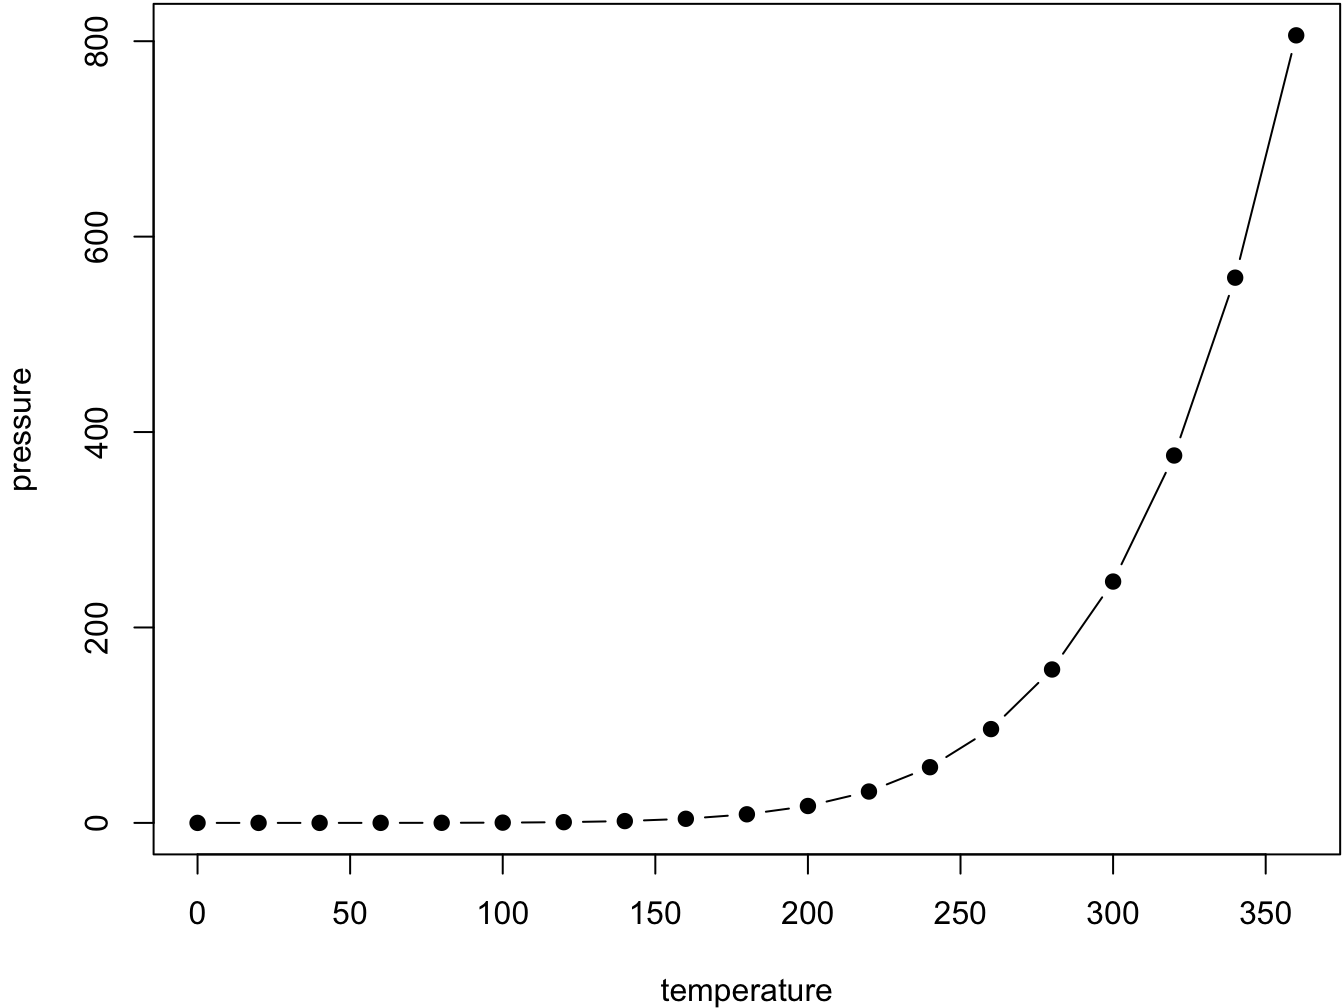
\includegraphics[width=0.8\linewidth]{bookdown-demo_files/figure-latex/nice-fig-1} 

}

\caption{Here is a nice figure!}\label{fig:nice-fig}
\end{figure}

Reference a figure by its code chunk label with the \texttt{fig:} prefix, e.g., see Figure \ref{fig:nice-fig}. Similarly, you can reference tables generated from \texttt{knitr::kable()}, e.g., see Table \ref{tab:nice-tab}.

\begin{Shaded}
\begin{Highlighting}[]
\NormalTok{knitr}\SpecialCharTok{::}\FunctionTok{kable}\NormalTok{(}
  \FunctionTok{head}\NormalTok{(iris, }\DecValTok{20}\NormalTok{), }\AttributeTok{caption =} \StringTok{\textquotesingle{}Here is a nice table!\textquotesingle{}}\NormalTok{,}
  \AttributeTok{booktabs =} \ConstantTok{TRUE}
\NormalTok{)}
\end{Highlighting}
\end{Shaded}

\begin{table}

\caption{\label{tab:nice-tab}Here is a nice table!}
\centering
\begin{tabular}[t]{rrrrl}
\toprule
Sepal.Length & Sepal.Width & Petal.Length & Petal.Width & Species\\
\midrule
5.1 & 3.5 & 1.4 & 0.2 & setosa\\
4.9 & 3.0 & 1.4 & 0.2 & setosa\\
4.7 & 3.2 & 1.3 & 0.2 & setosa\\
4.6 & 3.1 & 1.5 & 0.2 & setosa\\
5.0 & 3.6 & 1.4 & 0.2 & setosa\\
\addlinespace
5.4 & 3.9 & 1.7 & 0.4 & setosa\\
4.6 & 3.4 & 1.4 & 0.3 & setosa\\
5.0 & 3.4 & 1.5 & 0.2 & setosa\\
4.4 & 2.9 & 1.4 & 0.2 & setosa\\
4.9 & 3.1 & 1.5 & 0.1 & setosa\\
\addlinespace
5.4 & 3.7 & 1.5 & 0.2 & setosa\\
4.8 & 3.4 & 1.6 & 0.2 & setosa\\
4.8 & 3.0 & 1.4 & 0.1 & setosa\\
4.3 & 3.0 & 1.1 & 0.1 & setosa\\
5.8 & 4.0 & 1.2 & 0.2 & setosa\\
\addlinespace
5.7 & 4.4 & 1.5 & 0.4 & setosa\\
5.4 & 3.9 & 1.3 & 0.4 & setosa\\
5.1 & 3.5 & 1.4 & 0.3 & setosa\\
5.7 & 3.8 & 1.7 & 0.3 & setosa\\
5.1 & 3.8 & 1.5 & 0.3 & setosa\\
\bottomrule
\end{tabular}
\end{table}

You can write citations, too. For example, we are using the \textbf{bookdown} package \citep{R-bookdown} in this sample book, which was built on top of R Markdown and \textbf{knitr} \citep{xie2015}.

\hypertarget{elements-of-machine-learning}{%
\chapter{Elements of Machine Learning}\label{elements-of-machine-learning}}

In a minimalism style, machine learning refers to how computers can ``learn'' by finding patterns in data and using them to make predictions. Mathematically, given a real-valued output \(y\) and predictors vector \(X\) containing \(p\) variables, we assume a general function \(f\) to describe \(y\):

\begin{equation} 
y = f(X) + \epsilon
\label{eq:ml01}
\end{equation}

Where, \(f\) is a fixed but unknown function, and \(\epsilon\) is a zero-mean random error term, which is supposed to be independent of \(X\).

The core of machine learning is a suite of data-driven algorithms for estimating \(f\). ML is based on {\emph{statistical learning theory}} to design models to understand patterns and employs {\emph{optimization algorithms}} to train the model to ``learn'' the pattern using input data.

The foundation of practical machine learning is the data. Data drives everything else. The model can not learn much pattern without enough data and could even have biased behaviour if the data quality is poor. In contrast, with substantial data, the machine learning model could achieve impressive results beyond expectation. A vivid example is to check the google's search engine - it is machine learning algorithm under the hood.

\begin{quote}
``All models are wrong, but some are useful.'' - George E.P. Box
\end{quote}

\hypertarget{linear-regression}{%
\section{Linear Regression}\label{linear-regression}}

Linear regression adopts a linear function\(f^{Linear}\) to equation \eqref{eq:ml01} with learnable model parameters \(\beta^T =(\beta_0,\beta_1,...,\beta_p) \in (p,1)\):

\begin{equation} 
y = \beta^T X + \epsilon  
\label{eq:lm01}
\end{equation}

Here we assume the first column of \(X\) is all ones as an ``intercept feature'' and thus \(\beta_0\) corresponds to the intercept term.

The model given by \eqref{eq:lm01} defines the {\emph{population regression line}}, which is the best linear approximation to the true relationship between \(X\) and \(u\). The population regression line is unobserved and we have access to a set of sample observations to compute an sample-based estimate line. Fundamentally, we apply a standard statistical approach of using information from a sample to estimate characteristics of a large population. Here the linear regression focus on the estimate of coefficient \(\hat{\beta}\).

The most popular estimation method is {\emph{least squares}}, also known as Ordinary Least Squares (OLS). OLS regression is an estimated model based on sample data in which we pick the coefficients \(\hat{\beta}\) to minimize the residual sum of squares (RSS):

\begin{equation} 
RSS(\beta) = \sum_{i=1}^N (y_i - f(x_i))^2 = (y-X\beta)^T (y-X \beta)  
\label{eq:lmrss}
\end{equation}

To minimize \eqref{eq:lmrss}, we differentiate the term with respect to \(\beta\) and obtain:

\[
\frac{\partial RSS}{\partial \beta} = -2X^T (y - X \beta) \\
\frac{\partial RSS}{\partial \beta \partial \beta^T} =  2 X^TX
\]

Assuming that \(X\) has full column rank, hence \(X^TX\) is positive definite leading to optimality, we thus could set the first derivative to zero to get the \(\hat{\beta}\):

\[
X^T (y - X \beta) = 0  \\
\Rightarrow  X^T y  =  X^T X \hat{\beta}
\]

We thus solve the unique solution:

\begin{equation} 
\hat{\beta} = (X^TX)^{-1} X^T y
\label{eq:lmbeta}
\end{equation}

Please note all this derivation makes no assumptions about the validity of model - it simply finds the best linear fit to the data except from ensuring \(X\) is of full-rank. The non-full-rank case occurs most often when there is redundancy. A natural way to resolve the non-unique representation is to drop redundant columns in \(X\).

Lastly, since \(\hat{y}=X \hat{\beta}\), we could form the predictions
\begin{equation} 
\hat{y} = X \hat{\beta} = (X(X^TX)^{-1} X^T) y
\label{eq:lmyfit}
\end{equation}

We denote \(P=X(X^TX)^{-1} X^T\) which is projection matrix. Moreover, we could represent the residual \(\hat{\epsilon}\) with \(P\):
\begin{equation} 
\hat{\epsilon} = y - X \hat{\beta} = y - (X(X^TX)^{-1} X^T) y = (I_n - P) y
\label{eq:lmresid}
\end{equation}

Note \(Q=I_n - P\) is also a projection matrix. There are nice properties of {\emph{projection matrices}} that we will use in the subsequent sections:
\[
Q^T=Q; \;Q^2=Q
\]

\hypertarget{sampling-uncertainty-and-statistical-inference}{%
\subsection{Sampling Uncertainty and Statistical Inference}\label{sampling-uncertainty-and-statistical-inference}}

We infer from \eqref{eq:lmbeta} that both \(\hat{\beta}\) and \(\hat{Y}= X \hat{\beta}\) are linear transformations of \(y\) as random variables. If we had collected different sample data of size \(n\), we would to be sure have different estimates, due to {\emph{sampling uncertainty}}. We want to quantify this uncertainty by using {\emph{sampling statistics}} and essentially get more control of our estimate coefficient \(\hat{\beta}\). Furthermore, the inclusion of uncertainty measure such as standard error enables us to conduct statistical inference.

To pin down the sampling properties of \(\hat{\beta}\), we include supplementary assumptions including {\emph{uncorrelated residual}}, {\emph{constant variance of residual \(\sigma^2\)}}, and additionally {\emph{\(X\) is non-random}}. Based on the assumption, we infer the variance of \(y\):

\begin{equation} 
Var(y)=\sigma^2 I_n
\label{eq:lmyvar}
\end{equation}

We could then derive the expectation of residual sum of squares (RSS):

\[
RSS = Y^T(1-P)Y  \\
\Rightarrow  E[ Y^T(1-P)Y ] = (n-p) \sigma^2
\]

Hence we get the unbiased estimate of variance \(\hat{\sigma}^2 = \frac{RSS}{n-p}\). We next derive the variance-covariance matrix of the \(\hat{\beta}\) using equation \eqref{eq:lmyvar}:
\[
\begin{aligned}
Var( \hat{\beta}) &= Var( X(X^TX)^{-1} X^T ) \\&= X(X^TX)^{-1} X^T Var(y) (X(X^TX)^{-1} X^T)^T \\&=\sigma^2 (X^TX)^{-1}
\end{aligned}
\]
Therefore, the uncertainty in individual estimate \(\beta_j\) is quantified by its {\emph{standard error (\(SE\))}}
\[
\begin{aligned}
SE(\beta_j) = \sqrt{ \frac{\sigma}{ (X^TX)^{-1}_{jj} }}
\end{aligned}
\]

\hypertarget{rethinking-the-unbiasedness-of-ols}{%
\subsection{Rethinking the Unbiasedness of OLS}\label{rethinking-the-unbiasedness-of-ols}}

We require a property of unbiasedness for estimator \(\hat{B}\). Unbiased estimator does not systematically over- or under-estimate the true parameter \(B\).

Consider the decomposition of mean squared error of an estimator \(\tilde{\theta}\) in estimating \(\theta\):

\[
\begin{aligned}
MSE(\tilde{\theta}) &= E[ \tilde{\theta} - \theta ]^2 \\
                    &= Var( \tilde{\theta} ) +  [E( \tilde{\theta} ) - \theta ]^2
\end{aligned}
\]

Here the first term \(Var( \tilde{\theta} )\) is the variance, while the second term \([E( \tilde{\theta} ) - \theta ]^2\) is the squared bias.

The Gauss-Markov (GM) theorem implies that the least squares estimator has the smallest mean squared error (MSE) of all {\emph{linear estimators with no bias}} (⚠️ pay attention to the ``no bias'' here). However, there may well exist a biased estimator with smaller mean squared error. Such an estimator would {\emph{trade a little bias for a larger reduction in variance}}. Put bluntly, {\emph{biased estimates are commonly used}} for better out-of-sample performance (i.e., less MSE in test set). In reality, any method that shrinks or sets to zero some of the least squares coefficients may result in a biased estimate.

\hypertarget{assumptions-of-linear-regression-and-violation-implications}{%
\section{Assumptions of Linear Regression and Violation Implications}\label{assumptions-of-linear-regression-and-violation-implications}}

The question for the assumption of linear regression is ill-posed and requires more context as we need to specify the desired properties that we want the linear model to hold. Hence, we start with the standard assumptions that guarantee the above GM theorem to hold for OLS regression estimate:
1. There exists an additive linear model for \((X, Y)\) as equation \eqref{eq:ml01},
\[
Y= X \beta + \epsilon
\]
Where, \(\beta\) and \(X\) are {\emph{non-random}} while the randomness stem from \(\epsilon\)

\begin{enumerate}
\def\labelenumi{\arabic{enumi}.}
\setcounter{enumi}{1}
\item
  Zero Expected Mean of Residual: \(E[ \epsilon_i] = 0\)
\item
  Homoscedasticity: Constant Variance of Residual: \(Var(\epsilon_i)=\sigma^2 < \infty\)
\item
  Uncorrelated Residual Error: \(Cov(\epsilon_i, \epsilon_j)=0, \; \forall i\neq j\)
\end{enumerate}

Furthermore, if the error terms are 5. normally distributed and 6.identically and independently distributed (i.i.d.), we could infer that the OLS estimator becomes the Maximum Likelihood Estimation (MLE).

\hypertarget{problem-1-non-linearity-of-the-data}{%
\subsection*{Problem 1: Non-linearity of the Data}\label{problem-1-non-linearity-of-the-data}}

The linear regression model assumes that there is a straight-line relationship between the predictors and the response. If the true relationship is far from linear, then all of the conclusions that we draw from the fit are suspect.

🔍 \emph{Residual plots} are a useful visualization tool for identifying non-linearity. Given a fitted linear regression model, we can plot the residuals, \(e_i = y_i - \hat{y_i}\), versus the predictor \(x_i\). In the case of a multivariate regression model, we can plot the residuals versus the fitted values \(\hat{y_i}\). Independence assumption implies no discernible pattern. The presence of a pattern may indicate a problem with some aspect of the linear model. For instance, if residuals exhibit a clear U-shape, which provides a strong indication of non-linearity in the data.

\hypertarget{problem-2-correlation-of-error-terms}{%
\subsection*{Problem 2: Correlation of Error Terms}\label{problem-2-correlation-of-error-terms}}

An important assumption of the linear regression model is that the error terms \({\epsilon_i}\) are uncorrelated. Intuitively, if the errors are uncorrelated, then the fact that \(epsilon_i\) is positive provides little or no information about the sign of \(\epsilon_{i+1}\). One counterexample is to think about double a set of training observations \((X, y)\), as \(X_{Copy} = [X;X], y_{Copy}=[y;y]\).

The standard errors that are computed for the estimated regression coefficients or the fitted values are based on the assumption of uncorrelated error terms. If in fact there is correlation among the error terms, then the estimated standard errors will tend to {underestimate} the true standard errors. As a result, confidence and prediction intervals will be narrower than expected.

Such residual correlations frequently occur in the context of {time series data}, which consists of observations for which measurements are obtained at discrete points in time. There is the issue of {residual \href{https://en.wikipedia.org/wiki/Autocorrelation}{autocorrelation}} - tracking in the residuals that adjacent residuals may have similar values.

In general, the assumption of uncorrelated errors is extremely important for linear regression as well as for other statistical methods, and good experimental design is crucial in order to mitigate the risk of such correlations.

\hypertarget{problem-3-outliers}{%
\subsection*{Problem 3: Outliers}\label{problem-3-outliers}}

An outlier is a point which is far from the value predicted by the model. Outliers can arise for a variety of reasons, such as incorrect data collection. They are quite common in real dataset.

Residual plots can be used to identify outliers. If we believe that an outlier has occurred due to an error in data collection, then one solution is to simply remove the observation. Shrewd care and revised assumptions should be taken when removing outliers, since an outlier may instead indicate a deficiency with the model, such as a missing predictor. 2008 global financial crisis is a data point that needs justification to be discarded as outlier.

\hypertarget{problem-4-collinearity}{%
\subsection*{Problem 4: 💥Collinearity}\label{problem-4-collinearity}}

Collinearity refers to the situation in which a group of variables are closely related to one another. The presence of collinearity can pose problems in the regression context, since it can be difficult to separate out the individual effects of collinear variables on the response. Collinearity reduces the accuracy of the estimates of the regression coefficients, it causes the standard error for \(\hat{\beta_j}\) to grow.

🔍 {Correlation matrix of the predictors} is a simple way to detect collinearity. Unfortunately, not all collinearity problems can be detected by inspection of the correlation matrix: it is possible for collinearity to exist between three or more variables even if no pair of variables has a particularly high correlation - this is called {\emph{multicollinearity}}.

There are in two practical solutions to the problem of collinearity. The first, and more straightforward one, is to {\emph{drop}} one of the problematic variables from the regression. The second solution is to {\emph{aggregate}} the collinear variables together into a single composite predictor. For example, apply \href{https://en.wikipedia.org/wiki/Principal_component_analysis}{PCA} (Principal Component Analysis) approach to model the highly correlated features group and extract the first PC component as the representative indicator.

\hypertarget{conclusion}{%
\section{Conclusion}\label{conclusion}}

Linear models were largely developed in the precomputer age of statistics, but there are still robust baseline model to apply in today's computer era. They are simple and often provide an adequate and interpretable description of how the inputs affect the output. For prediction purposes they can sometimes outperform fancier nonlinear models, especially in situations with small numbers of training cases, low signal-to-noise ratio or sparse data.

\hypertarget{modern-factor-investing}{%
\chapter{Modern Factor Investing}\label{modern-factor-investing}}

\begin{quote}
We give an overview of modern factor investing in this chapter. It is intended to be an introductory chapter to help readers get familiar with the quantitative finance framework. This chapter is adapted from our Webinar series {\emph{Modern Factor Investing: Past, Present, Future}}.
\end{quote}


\includegraphics[width=1\linewidth]{images/chapter3/nyc}

Over the last 50 years, academic researchers have made major breakthroughs in advancing classical practice in finance, from fundamental analysis to scientific quantitative research. These include portfolio theory, corporate finance, financial engineering of derivative instruments, and many other applications pertaining to financial markets overall. One of the foundational pillar is the advances in capital market theory in the context of descriptive equilibrium propositions in terms of the risk/return tradeoff and the linear factor model to explain the expected asset price, beginning with William F. Sharpe and the {\emph{Capital Asset Pricing Model (CAPM)}} \citep{sharpe1964capital}. Many related academic developments provided rich asset pricing insight, including {\emph{Arbitrage Pricing Theory (APT)}} \citep{ross1976arbitrage}, market efficiency proposition, market anomalies such as the {\emph{Fama and French factor model}}, and behavioral finance. These altogether gave birth to a new investment paradigm - {\emph{factor investing}} - this is where classical financial textbooks end.

The saying, ``change is the only constant in life'' is attributed to the Greek philosopher, Heraclitus around 500BC. This is even more prominent to the capital market. The evolution of financial market keeps testing the efficacy of the factor theory and model. Ever since the 2008 global financial crisis, we observe an irreversible performance decay of the traditional factor model that is solely based on conventional data and linear framework. In academia, there is also a replication crisis (or credibility crisis) raging on as ``most claimed research findings in financial economics are likely false.'' \citep{harvey2016and}

Perhaps the Fourth Industrial Revolution has already come, and \emph{\href{https://www.gsb.stanford.edu/insights/andrew-ng-why-ai-new-electricity}{``AI is the new electricity''}}. During the trend, factor models and strategies have not remained static. Factor models and investment strategies evolve gradually over time, reflecting the evolution of capital markets and advances in data science theories, data availability, and investment practice. One of the exciting current innovation efforts in factor investing focus on exploiting new unstructured data sources - the {\emph{alternative data}}, applying new data science modeling techniques - {\emph{machine learning}} - this is where the modern factor investing starts.

\hypertarget{overview-of-factor-investing}{%
\section{Overview of Factor Investing}\label{overview-of-factor-investing}}

\begin{quote}
One of our central themes is that if assets are priced rationally, variables that are related to average returns, such as size and book-to-market equity, must proxy for sensitivity to common (shared and thus undiversifiable) risk factors in returns --- Fama and French (1993)
\end{quote}

The question of what drives asset returns has been a staple of neoclassical finance and remains a holly grail. The factor model emerged and became a foundation of asset pricing theory in the 1960s (Lintner, 1965; Mossin, 1966; Sharpe, 1964 and Treynor, 1961). In general, Factor can be defined as any underlying characteristic relating a group of assets (e.g., equity, bond) that is linearly significant in explaining their return and risk.

Factor investing refer to the general use of factors in the investment process. It is trustworthily a quantitative paradigm in investment where factor models renders return prediction signal, forecast expected asset risk, and drive asset allocation decisions by using the tradable factor portfolios. Practically, factor-driven investment strategies such as smart beta products amount to \$800 billion AUM worldwide (Johnson 2018) --- yes, we are talking about a magnificent investment topic that may affect everyone's saving pension.

Fundamental factors are the bedrock of modern investment management and have served the needs of investors for a long time. For equities, in addition to countries and industries, fundamental factors documented through empirical research and used extensively in portfolio management include value, size, momentum, volatility, quality, yield, growth, and liquidity. A similar set of common macro drivers has been identified and used across asset classes, including equity, rates, credit, and real assets.

Now that we have the mathematical formulation, we delve into the granular categories of the factors:

\begin{itemize}
\item
  \textbf{Beta factors} --- factors corresponding to \(f_t\) are generally referred as ``risk premia factors'', which have reflected exposure to sources of systematic risk and are supposed to earn a persistent significant risk-compensated premium over long periods ({\emph{if all model assumptions work\ldots{}}}).

  In practice, they are called ``beta factors'' or ``style factors'' to denote that they are the drivers of systematic return and risk of assets. Furthermore, they are usually associated with the systematic risk that is inherent in market.

  Here the risk premium reward could be thought as selling insurance products to Mr.~Market. You undertake the risk to receive a positive reward on average in the long-term, when the risk does happen, Mr Market will come to you for coverage and you suffer a realized loss that should be well anticipated. If you believe the game is fair then you agree with the philosophy of \href{https://www.investopedia.com/terms/p/passiveinvesting.asp}{passive investing}.
\item
  \textbf{Alpha factors} --- some other factors fall into the \(\alpha_{i,t}\) term as they do not explain the risk well (e.g., {\emph{they are not volatile}}) and can not be included into the linear terms, yet they do earn persistent return over time with some predictive value to result in \(\alpha_{i,t} \neq 0\).

  Alpha factor model are designed to forecast excess return of stocks. If return distribution is characterized by the expected return and the standard deviation, it is often the expected return predicted by alphas that determines whether we buy or sell, overweight or underweight, and the standard deviation driven by betas that determines the size of the portfolio allocations to hedge the undesirable systematic risk - this is the monologue of hedge funds or active investment.

  Efficient market theory forbids the existence of alpha and the academia call them {\emph{``anomaly''}}, however, hedge fund active managers rely on them and {\emph{some of them seem to live well}}. They are often called ``signal'' by practitioners to distinguish from the beta risk premia factors.

  The alpha signals are often proprietary and highly guarded, reflecting creativity as well as superior systems. It is the most important differentiator within the investment firm.
\end{itemize}

\hypertarget{years-of-factor-investing-a-literature-review}{%
\section{50 Years of Factor Investing: A Literature Review}\label{years-of-factor-investing-a-literature-review}}

Factor research has been prevalent for over 40 years. The oldest and most well-known model of stock returns is the Capital Asset Pricing Model (CAPM), which is in essence a single-factor model with market as the sole factor (see Sharpe 1964). In other words, the expected return to any stock could be viewed as a function of its beta factor loading to the market . This won William Sharpe a Nobel Prize.

\hypertarget{limitedness-of-classical-factor-model-and-the-factor-zoo}{%
\section{Limitedness of Classical Factor Model and the Factor Zoo}\label{limitedness-of-classical-factor-model-and-the-factor-zoo}}

The enduring success of fundamental factors stems from the fact that they are guided by academic theory, and, importantly, are supported by empirical evidence and reflect investment practice, i.e., they make money. However, the story of factors turn into a horror fiction ever since the 2008 Global Financial Crisis. It is not only that some well-acclaimed factors that outperform in the past start to underperform, but also there are some lurking \href{https://en.wikipedia.org/wiki/Black_swan_theory}{black swan events} that causing extreme outliers where the model could fail drastically. In statistics this is usually associated with the {\emph{heavy-tailed}} distribution and we could sometimes remove or winsorize those data points as outliers when fitting a model. Nevertheless, in reality these outliers may mean you are doomed all at once.

To make a concrete example, lets remember David Viniar's, once the CFO of Goldman Sachs, famous explanation when Goldman's flagship GEO hedge fund had lost 27\% in 2007: \emph{``We were seeing things that were 25-standard deviation moves, several days in a row.''}. One commentator wryly noted:

\begin{quote}
That Viniar. What a comic. According to Goldman's mathematical models, August, Year of Our Lord 2007, was a very special month. Things were happening that were only supposed to happen once in every 100,000 years. Either that \ldots{} or Goldman's models were wrong (Bonner, 2007b).
\end{quote}

A direct implication is that the normality assumption of linear models does not hold in financial market, thereby significantly weakening the {\emph{statistical inference}} power in quantitative fiance. The p-value and relevant test statistics should thus be interpreted with extreme caution or neglected altogether. We empirically recommend the latter.

More importantly, the underlying linearity assumption itself is an unrealistic assumption and we have witness a great amount of evidence on {\emph{non-linearity}} breaking this fundamental assumption. One of the straightforward counterexample is the interaction effect as one factor's contribution to the asset's expected return may rely on other factors. Furthermore, there could be more complex pattern that certain factor exerts on the asset return and risk. You should forget about the theoretical unbiasedness credit to linear model when entering the quantitative finance.

Another interesting trend is the ``factor zoo'' \citep{harvey2019census}, which refers to a metaphor for the growing number of investment factors proposed by both academics and practitioners. Not considering the less famous journals or the mysterious industry, there are already hundreds of factors claimed to be effective and published in top academic journals.\\

\begin{figure}
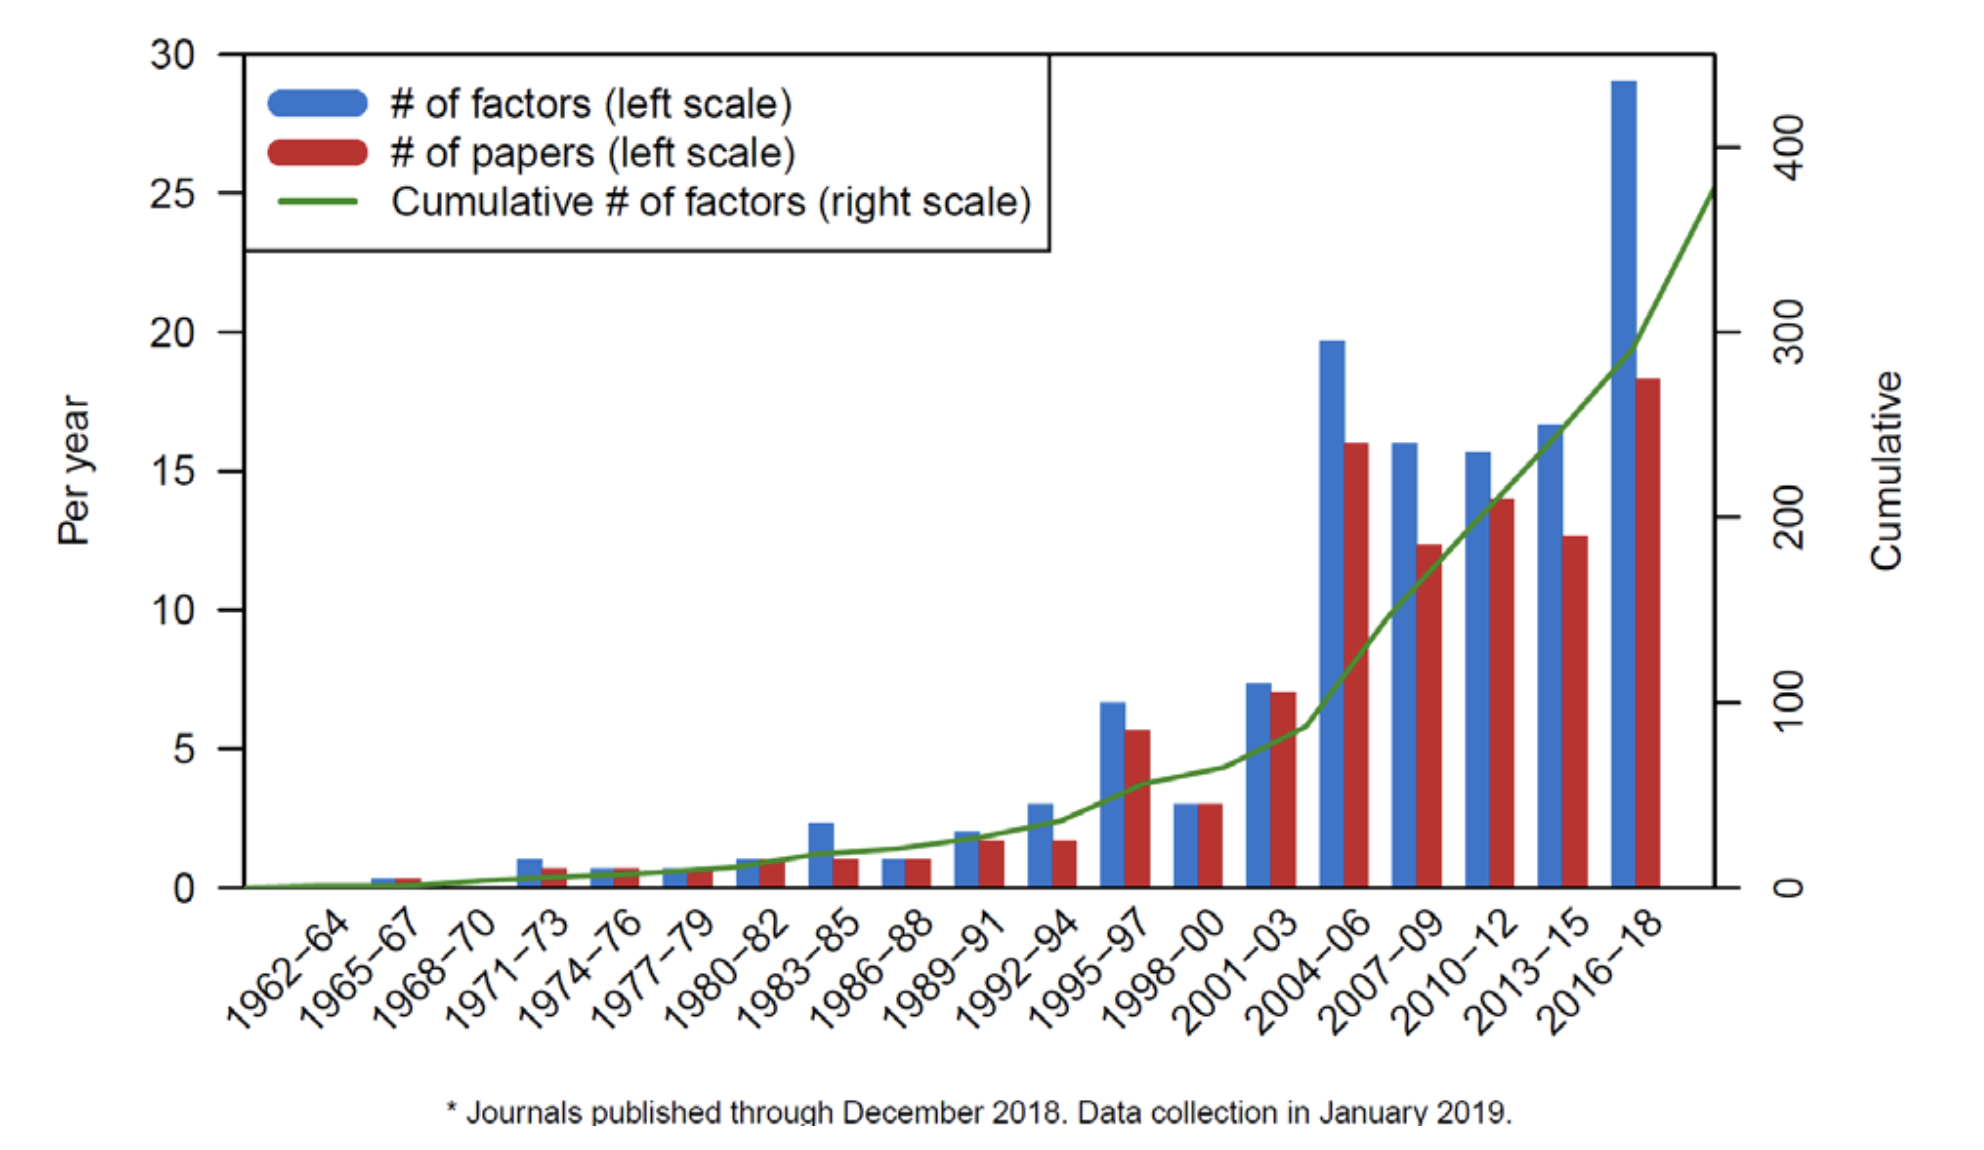
\includegraphics[width=0.9\linewidth]{images/chapter3/factor_zoo} \caption{Out of control factor production, (Harvey, 2019)}\label{fig:unnamed-chunk-2}
\end{figure}

This point out to the multiple testing problem: \emph{with so many factors tried, some will appear ``significant'' purely by chance}, and further indicates the peril of data mining, which may or may not be intentional. From a data science perspective, this also leads to the {\emph{high-dimension}} nature of the modern factor investing: we now have a ``zoo'' of available factor candidates and the traditional OLS linear regression is incompetent.

Therefore, the linear model is at most a compromise in facing of the low noise-to-signal ratio data in financial market.

\hypertarget{modern-factor-investing-in-the-big-data-and-machine-learning-trend}{%
\section{Modern Factor Investing in the Big Data and Machine Learning Trend}\label{modern-factor-investing-in-the-big-data-and-machine-learning-trend}}

What is Big Data? A wide array of information sensing devices as well as the cloud service technique has led to an exponential growth in available big datasets. Starting from handheld mobiles, cameras, microphones, Internets, digitalised map, Internet of Things (IoT), to LiDAR (Light Detection and Ranging) sensors and satellite imaging. The amount of data that the world collects has experienced explosive growth. The rapid development of informative technologies has paved the way for a transition to digital world.

The rapid advancement in the Internet and social media sectors has far reaching effects not only on our day to day lives; but also, for finance researchers and investors. Quantitative finance is no longer a subclass of finance but arguably the whole finance is evolving into a data-driven scientific subject. There comes a fashionable term in the finance domain - {\emph{alternative data}}.

Alternative data is data not typically used by researchers and model builders and can be sourced from a kaleidoscope of data sources ranging from text, audio, image, graph, etc. These data sets typically have minimal aggregation and processing making them more {\emph{difficult}} to access and use. In the last several years, we have seen an explosion in the availability of new alternative data sources.

\begin{itemize}
\item
  Some of the alternative data sets are market data that were previously difficult to access (e.g., analyst forecasts, insider transactions, options trading information, credit default swaps, and hedge fund positions). These data sets are available in numerical format and can be sourced from commercial vendors.
\item
  Other new data sets come in new atypical formats (e.g., text, audio, and video), and they can only be extracted from internet sites and social media. Investors may gain additional insights by processing and understanding the information contained in unstructured alternative data sets such as news reports, product reviews, employee reviews, job postings, regulatory filings, call transcripts, satellite images, etc.
\end{itemize}

The new formats require new modeling techniques and powerful computers to extract information. Innovations in information technology such as cloud computing and bespoke microprocessors provide the computational firepower necessary to apply {\emph{machine learning}} and other computationally intensive data science techniques on the new unstructured alternative data sets.

{\emph{Natural language processing (NLP)}} is one of the most exciting frontiers to bring alternative value to the factor investing framework. In essence, we could now leverage deep-learning based NLP model to extract value from text data in the financial domain. Financial sector accumulates large amount of financial communication text. It is only the recent machine learning breakthrough of general {\emph{Natural Language Understanding (NLU)}} language model such as BERT \citep{devlin2018bert} that makes the unstructured text data become a goldmine to generate value for quantitative finance. Due to its unique data source, NLP-based factors tend to have a merit of {\emph{being orthogonal to existing fundamental factors}} with less multicollinearity issue. It is thus pivotal to note that NLP-based factors could actually complement the existing factors, instead of the disrupting them overall. We will give a detailed introduction of Financial NLP in the latter sections, which well deserve a chapter in its own right.

In another vein, much of the efforts have been focused on employing modern high-dimensional machine learning techniques to better model the asset returns now given the affluence of data source. Applying machine learning routines to financial data has been implicitly motivated by the AFA (American Finance Association) presidential address of Cochrane (2011), who suggests that in the presence of a vast collection of noisy and highly correlated return predictors, there is a need for other methods beyond cross-sectional linear regressions. Indeed, {\emph{machine learning}} offers a natural and theoretical-sound way to accommodate a high-dimensional predictor set and flexible functional forms, and it employs ``regularization'' methods to select models, mitigate overfitting biases, and uncover complex patterns and hidden relationships.

There has been an emerging body of pioneer academic work that reports phenomenal investment profitability based on signals generated by machine learning methods, let alone the long data science enthusiasm from investment industry. A funny observed phenomenon to echo this trend is that nowadays Machine Learning PhDs are more likely to land a researcher job in quantitative Hedge Funds than those pure Finance PhDs.

We list some most influential papers here \ref{tab:ML-factor-tab} as a roadmap of the recent modern factor investing. The predictors column refer to the input features the research use to predict the stock returns, where Firm stands for typical firm-level factors and Macro represents the macro indices. In the forthcoming sections we will deep dive into some most representative ones (e.g., IPCA) alongside introducing the corresponding machine learning algorithm.

\begin{table}

\caption{\label{tab:ML-factor-tab}Factor machine learning papers, up till December 2021}
\centering
\begin{tabular}[t]{llllll}
\toprule
ML.Models & Linearity & Factor.Model & Predictors & Paper & Name\\
\midrule
Linear Shrinkage & Linear & Pricing Kernel & Firm & NKS, 2020 & Shrinking the cross-section\\
IPCA & Linear & Beta Pricing & Firm & KPS, 2019 & Characteristics are covariances: A unified model of risk and return\\
Auto Encoder & Nonlinear & Beta Pricing & Firm & GKX, 2019 & Autoencoder asset pricing models\\
Reg Tree & Nonlinear & Reduced Form & Firm + Macro & GKX, 2020 & Empirical asset pricing via machine learning\\
GNN & Nonlinear & Pricing Kernel & Firm + Macro & CPZ, 2019 & Deep learning in asset pricing\\
\addlinespace
Transformer & Nonlinear & Residual Term & Firm & JMG, 2021 & Deep learning statistical arbitrage\\
\bottomrule
\end{tabular}
\end{table}

\hypertarget{chapter-conclusion}{%
\section{Chapter Conclusion}\label{chapter-conclusion}}

Given the plethora of factors and the inevitable data mining, many of the historically discovered factors would be deemed ``significant'' by chance.

\hypertarget{applications}{%
\chapter{Applications}\label{applications}}

Some \emph{significant} applications are demonstrated in this chapter.

\hypertarget{example-one}{%
\section{Example one}\label{example-one}}

\hypertarget{example-two}{%
\section{Example two}\label{example-two}}

\hypertarget{final-words}{%
\chapter{Final Words}\label{final-words}}

We have finished a nice book.

  \bibliography{book.bib,packages.bib}

\end{document}
